\begin{frame}{link-state advertisements (router)}
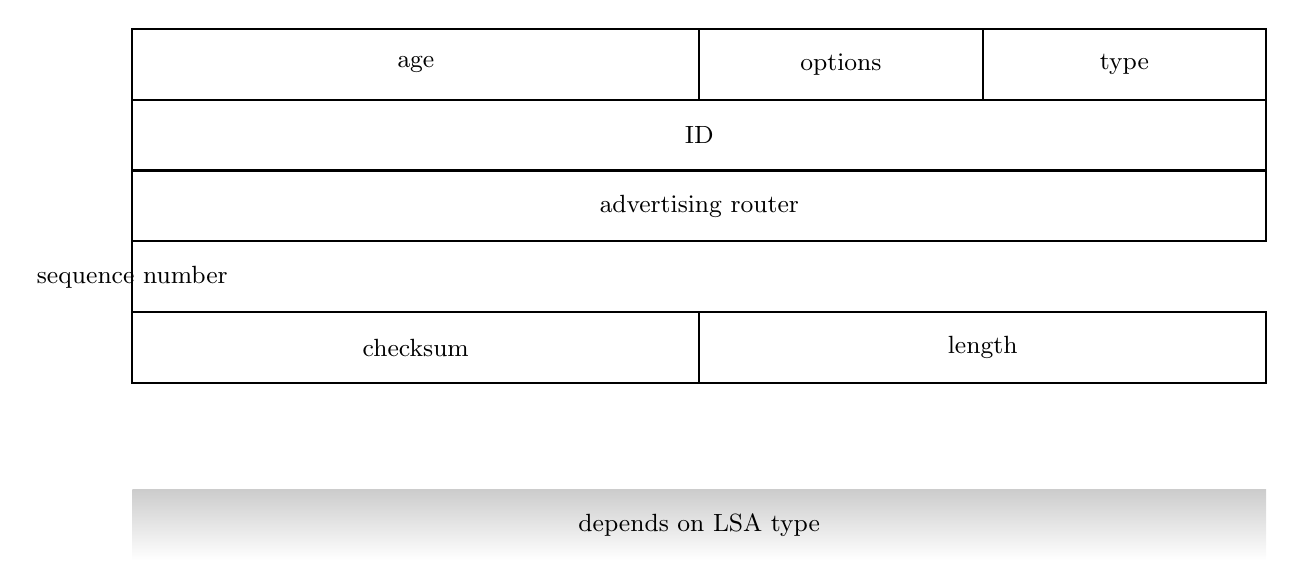
\begin{tikzpicture}
\tikzset{
    box/.style={draw,thick},
    label/.style={font=\small},
    label large/.style={},
    box label/.style={midway,font=\small,align=center},
    box label flags/.style={midway,font=\fontsize{8}{9}\selectfont,align=center},
    missing/.style={pattern=north west lines},
    length field/.style={alt=<3>{fill=red!10,very thick}},
    tos/.style={alt=<5>{fill=red!10,very thick}},
    %frag/.style={alt=<3>{fill=red!10,very thick}},
    ttl/.style={alt=<4>{fill=red!10,very thick}},
    addrs/.style={alt=<6>{fill=red!10,very thick}},
    type field/.style={alt=<2>{fill=red!10,very thick}},
    checksum/.style={alt=<6>{fill=red!10,very thick}},
}
\begin{scope}[x=0.45cm,y=0.9cm]
\draw[box] (0, 0) rectangle (16, -1)
    node[midway,label] {age};
\draw[box] (16, 0) rectangle (24, -1)
    node[midway,label] {options};
\draw[box] (24, 0) rectangle (32, -1)
    node[midway,label] {type};
\draw[box] (0, -1) rectangle (32, -2)
    node[midway,label] {ID};
\draw[box] (0, -2) rectangle (32, -3)
    node[midway,label] {advertising router};
\draw[box] (0, -3) rectangle (0, -4)
    node[midway,label] {sequence number};
\draw[box] (0, -4) rectangle (16, -5)
    node[midway,label] {checksum};
\draw[box] (16, -4) rectangle (32, -5)
    node[midway,label] {length};
\path[shading=axis,bottom color=white,top color=black!20] (0, -6.5) rectangle (32, -7.5)
    node[box label] {depends on LSA type};
\end{scope}
\end{tikzpicture}
\end{frame}

\begin{frame}{LSA sequences/ages}
    \begin{itemize}
    \item sequence number for getting correction version of LSAs
        \begin{itemize}
        \item some tricky rules to handle routers restarting (losing track of sequence number) and sequence number wraparound
        \end{itemize}
    \item maximum `age' for link-state advertisements
        \begin{itemize}
        \item typically minutes
        \item too-old LSAs not used for routing
        \item deliberately setting age = MaxAge used to invalidate LSAs
        \end{itemize}
    \end{itemize}
\end{frame}

\begin{frame}{LSA types}
\begin{itemize}
\item `router':
    \begin{itemize}
    \item list of links for router
    \item links = connect to other router or network
    \item links refer to ID numbers of network/router LSAs
    \item metrics for each link
    \end{itemize}
\item `network':
    \begin{itemize}
    \item list of routers for network
    \item different version of external and internal networks
    \end{itemize}
\item (later) `summary':
    \begin{itemize}
    \item part of support for \textit{areas}
    \item used when sysadmin doesn't want all routers processing whole network map
    \end{itemize}
\end{itemize}
\end{frame}
